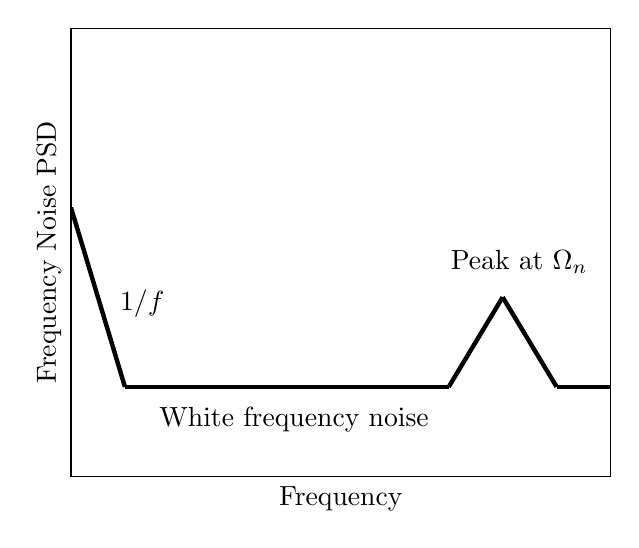
\begin{tikzpicture}
\begin{axis}[
xmin=0,
xmax=10,
ymin=0,
ymax=5, 
xlabel=Frequency,
ylabel=Frequency Noise PSD,
ticks=none,
samples=10]
\addplot[black, ultra thick, domain=1:7] (x, 1);
\addplot[black, ultra thick, domain=0:1] (x, 3-2*x);
\addplot[black, ultra thick, domain=7:8] (x, x-6);
\addplot[black, ultra thick, domain=8:9] (x, -x+10);
\addplot[black, ultra thick, domain=9:10] (x, 1);
\end{axis}     
\draw (0.5, 2.5) node [below right] {$1/f$};
\draw (4.7, 3) node [below right] {Peak at $\Omega_n$};
\draw (1, 1) node [below right] {White frequency noise};
\end{tikzpicture}